64. Постройте график функции $y=\cfrac{(x^2-4x+3)(x-1)}{|x-1|}.$ При каких $m$ прямая $y=m$ пересекает график функции в трёх точках?
ewpage

oindent65. Могут ли параболы на рисунке  быть графиками функций  $f(x)=ax^2+b_1x+c$ и $g(x)=cx^2+b_2x+a?$
$$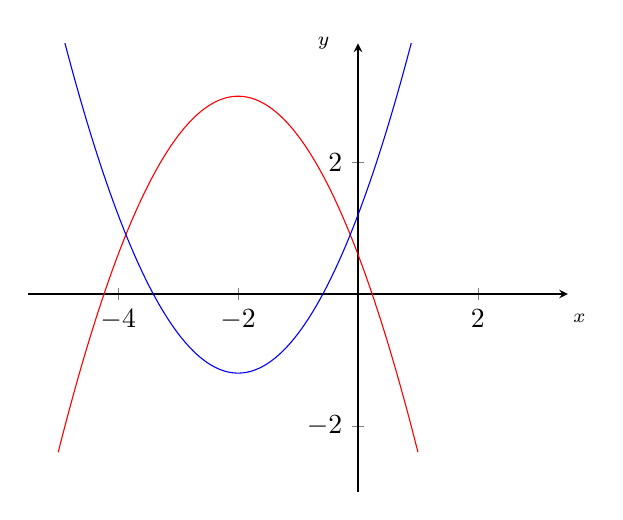
\begin{tikzpicture}[scale=1]
\begin{axis}[
    axis lines = middle,
    legend pos={south west},
    %xlabel = {$x$},
    %xlabel style={below right},
    %ylabel = {$y$},
    %title={$\text{Рис. 2}$},
    ymin=-3,
    ymax=3.8,
    xmin=-5.5,
    xmax=3.5,
    %xtick=\empty,
	%ytick=\empty,
    ]
	\addplot[domain=-5:1, samples=100, color=red] {-0.6*(x^2+4*x-1)};
	\addplot[domain=-5:1, samples=100, color=blue] {0.6*(x^2+4*x+2)};
%\addlegendentry{$\text{Рис. 1}$};
\end{axis}
\draw (3.75,5.7) node {\scriptsize $y$};
\draw (7,2.2) node {\scriptsize $x$};
\end{tikzpicture}$$
